\graphicspath{ {./resources/pid/} }
\documentclass[../templateLTHtwocol.tex]{subfiles}
\begin{document}

The objective of the agent is to complete a full 360 degrees helix. In the simulation environment, a circle is used for training, and convergence is measured against the Crazyflie trajectory to trace a helix. In figures \ref{fig:figpid1}, \ref{fig:figpid2}, and \ref{fig:figpid3} the output plot compares the tuned (output parameters from the algorithm) vs the default for test trajectory along X, Y and Z axis.

Hardware testing includes the two methods mentioned above. First, the relative positioning system uses the Flow deck, which shows a rougher point-to-point displacement, meanwhile, the absolute positioning using the Lighthouse shows a smoother performance. See figures \ref{fig:figpid4} and \ref{fig:figpid5} for more details.

Finally, figure \ref{pid_step_response:fig} shows the step responses, where tuned and default parameters have similar results. Therefore, we can conclude that the estimated model is approximated enough to the real, for more details table \ref{pid_step:table} presents more step response information. 


\begin{figure}[H]
	\centering
	\caption{Helix Test Results in Gym-Pybullet-Drones}
	\begin{subfigure}[b]{0.2\textwidth}
		\caption{X}
		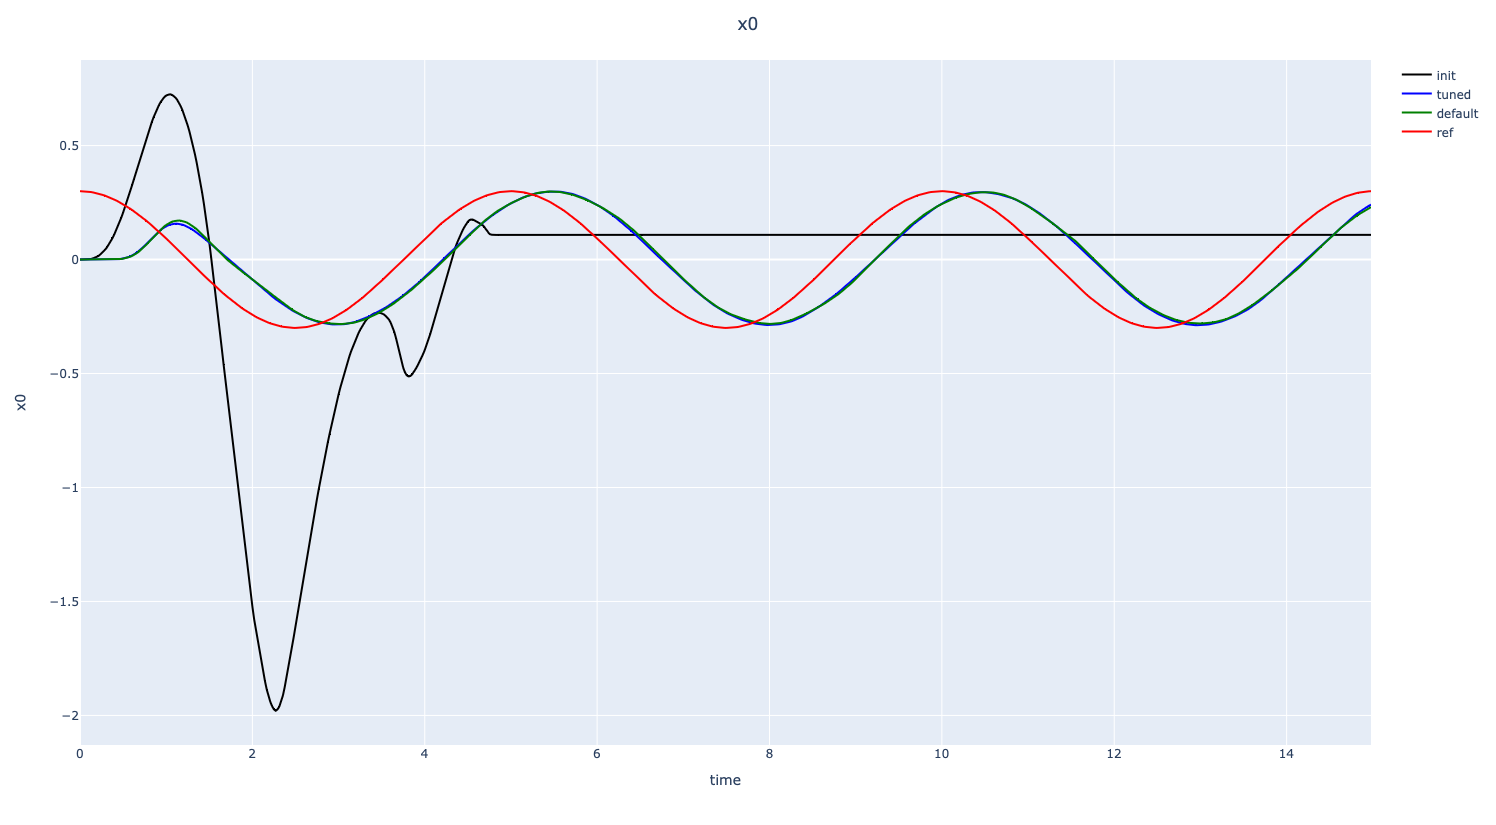
\includegraphics[width=\textwidth]{resources/pid/x0.png}
		\label{fig:figpid1}
	\end{subfigure}
	\hfill
	\begin{subfigure}[b]{0.2\textwidth}
		\caption{Y}
		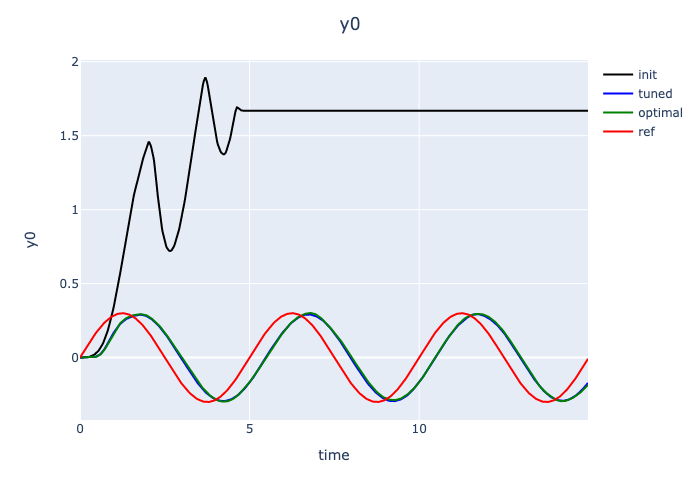
\includegraphics[width=\textwidth]{resources/pid/y0.png}
		\label{fig:figpid2}
	\end{subfigure}
	\hfill
	\begin{subfigure}[b]{0.2\textwidth}
		\caption{Z}
		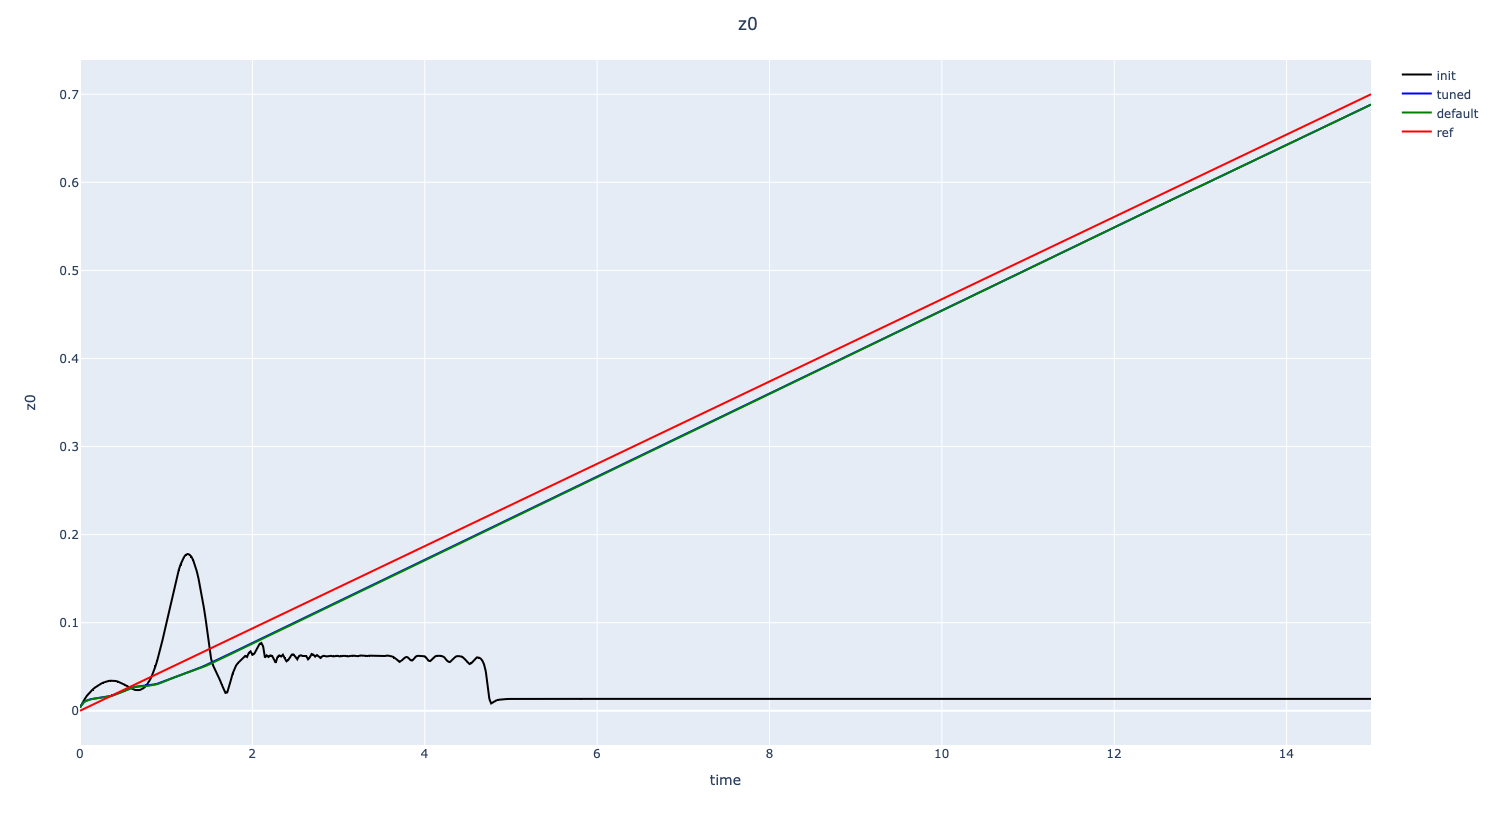
\includegraphics[width=\textwidth]{resources/pid/z0.png}
		\label{fig:figpid3}
	\end{subfigure}
	\hfill
	\begin{subfigure}[b]{0.2\textwidth}
		\caption{Step Response}
		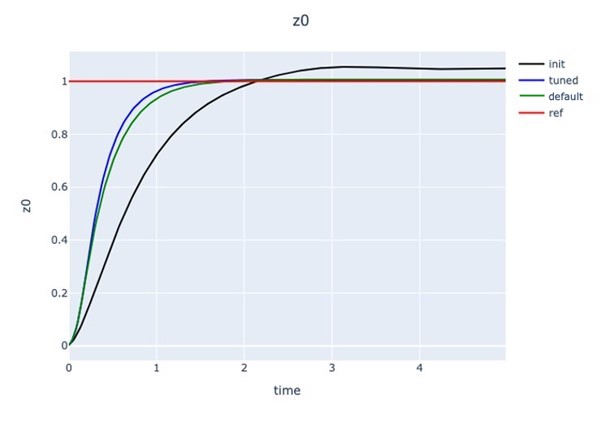
\includegraphics[width=\textwidth]{resources/pid/step_response_PID.jpg}
		\label{pid_step_response:fig}
	\end{subfigure}
\end{figure}

\begin{figure*}[h]
	\centering
	\caption{Helix - Hardware Results}
	\begin{subfigure}[b]{0.4\textwidth}
		\caption{Flow Deck (Relative Positioning)}
		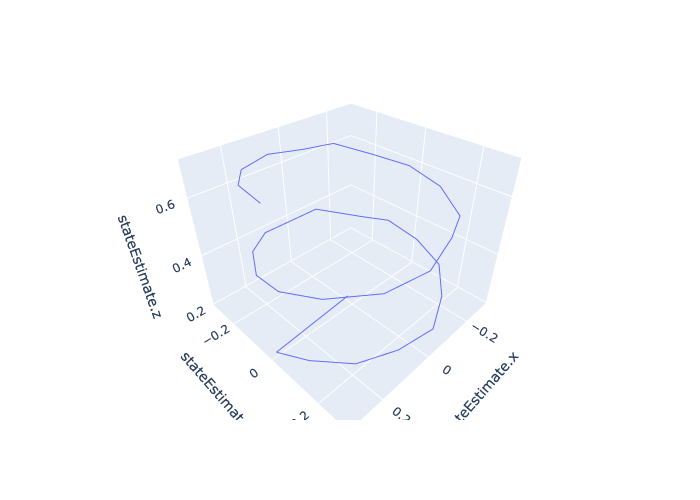
\includegraphics[width=\textwidth]{flowdeck.png}
		\label{fig:figpid4}
	\end{subfigure}
	\hfill
	\begin{subfigure}[b]{0.4\textwidth}
		\caption{Lighthouse Deck (Absolute Positioning)}
		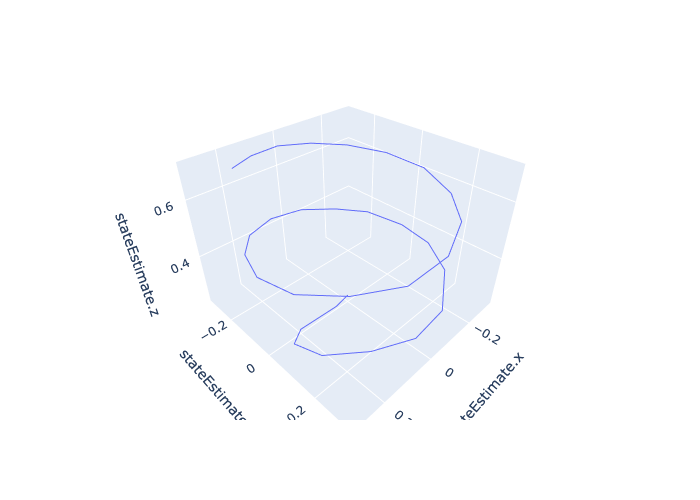
\includegraphics[width=\textwidth]{Lighthouse.png}
		\label{fig:figpid5}
	\end{subfigure}
\end{figure*}

\begin{table*}[h]
\caption{Step Response Characteristics - Randomly initialized vs Tuned vs Default }
\label{pid_step:table}
\centering
\begin{tabular}{|l|c|c|c|}
\hline
\textbf{Characteristics} & \begin{tabular}[c]{@{}l@{}} \textbf{Randomly Initialized} \\ \textbf{Params}\end{tabular} & \textbf{Tuned Params} & \textbf{Default Params} \\ \hline \hline
Rise Time (s)      & 1.557                                                                  & 0.649        & 0.7728         \\ \hline
Settling Time (s)   & 2.445                                                                  & 1.199        & 1.4028         \\ \hline
Overshoot       & 0.548                                                                  & 0.0373       & 0.1901         \\ \hline
Peak            & 1.0546                                                                 & 1.000        & 1.0067         \\ \hline
\end{tabular}
\end{table*}

\begin{table*}[h]
\caption{PID Tuning - Default vs Tuned Coefficients}
\label{pid_tab1:table}
\centering
\begin{tabular}{|c|l|c|c|c|c|c|c|}
\hline
\multirow{3}{*}{\textbf{Position Controller}} &                  & \textbf{kp\_xy} & \textbf{kp\_z} & \textbf{ki\_xy}    & \textbf{ki\_z}    & \textbf{kd\_xy} & \textbf{kd\_z} \\ \cline{2-8} 
                                              & \textbf{Default} & 0.4             & 1.25           & 0.05               & 0.05              & 0.2             & 0.5            \\ \cline{2-8} 
                                              & \textbf{Tuned}   & 0.364           & 1.169          & 0.052              & 0.052             & 0.234           & 0.586          \\ \hline
\multirow{3}{*}{\textbf{Attitude Controller}} & \textbf{}        & \textbf{kR\_xy} & \textbf{kR\_z} & \textbf{ki\_m\_xy} & \textbf{ki\_m\_z} & \textbf{kw\_xy} & \textbf{kw\_z} \\ \cline{2-8} 
                                              & \textbf{Default} & 70000           & 60000          & 0.0                & 500               & 20000           & 12000          \\ \cline{2-8} 
                                              & \textbf{Tuned}   & 64786.842       & 55531.579      & 0.0                & 599.666           & 17217.406       & 10330.444      \\ \hline
\end{tabular}
\end{table*}

\end{document}